%%%%%%%%%%%%%%%%%%%%%%%%%%%%%%%%%%%%%%%%%%%%%%%%%%%%%%%%%%%%%%%%%%%%%%%%%%%%%%%%
\chapter{Introduction}\label{ch:introduction}
%%%%%%%%%%%%%%%%%%%%%%%%%%%%%%%%%%%%%%%%%%%%%%%%%%%%%%%%%%%%%%%%%%%%%%%%%%%%%%%

%4th-review
\section{Motivation}
 

The type of traffic used for performing evaluation matters; this is a fact. Studies show that realistic Ethernet traffic provides different and variable load characteristics on routers\cite{harpoon-validation}, even with the same average bandwidth consumption, showing that constant traffic is not sufficient for complete technology validation. This conclusion indicates that tests which employ traffic generators with constant rates are not enough for complete validation of new technologies. Bursty traffic can cause packet losses and buffer overflows, impacting network performance and measurement accuracy\cite{burstiness-queue-lenght}. Small packets tend to degrade application performance\cite{comparative-trafficgen-tools}.  Furthermore, realistic traffic is essential on security research, such as for the evaluation of firewall middleboxes, studies on intrusion, and malicious workloads\cite{ditg-paper}. 

New networking scenarios such as \acrshort{SDN} and virtualized networks (\acrshort{NFV} and \acrfull{VNF}s) become harder to predict in terms of performance compared to hardware-based technologies, due to the multiple layers of software and platform parameters demanding validation in a broadening range of use cases~\cite{nfv-challenges}. Another critical question about the interaction between application- network has had the flow-oriented operation of SDN networks, in which each new flow arriving on an SDN switch demands further communication with the controller. Therefore the controller can be a bottleneck on the switches performance.  Also,  new types of traffic patterns introduced by \acrfull{IoT} and Machine-to-Machine (\acrfull{M2M}) communication\cite{machine2machine}  increase the complexity of the network traffic characterization, turning pre-defined models used by traffic generators obsolete. 

Furthermore, realistic traffic generators are essential security research, since the generation of realistic workloads is essential for evaluation of firewall middleboxes. It includes studies of intrusion, anomaly detection, and malicious workloads. By realistic, we refer to traffic that represents well the traffic features, such as protocols, payloads, and protocols, able to emulate benign and malicious workloads. 

Aiming to address these gaps, this dissertation introduces \acrfull{SIMITAR}, an auto-configurable network traffic generator. SIMITAR stands for \textit{SnIffing, ModellIng, and TrAffic geneRation}, which correspond to the main operation processes of the proposed framework.  SIMITAR has an application independent traffic model, that can represent a wide variety of scenarios. It also decouples the traffic modeling and packet-generation layer, using a factory design pattern, enabling its application on different scenarios, and technology update, via technology abstraction.  SIMITAR code and all scripts used in this paper are available at GitHub\cite{projeto-github} for validation, experiment reproducibility, and re-use purposes. 


\section{Related Work}


\begin{table*}[ht!]
    \centering
    \caption{Comparison of existing traffic generation tools.}
    \scalebox{0.80}{ 
    \begin{tabular}{ccccc}
        \hline
        \rowcolor[HTML]{9B9B9B} 
        \hline
        \textbf{Solution}     & \textbf{Auto-configurable} & \textbf{Realistic Traffic} & \textbf{Traffic Custumization} & \textbf{Extensibility} \\ \hline
        Harpoon     & yes              & yes               & yes                   & \textbf{no}   \\
        \rowcolor[HTML]{C0C0C0} 
        D-ITG                & \textbf{no}      & yes               & yes                   & \textbf{no}   \\
        Swing                & yes              & yes               & \textbf{no}           & \textbf{no}   \\
        \rowcolor[HTML]{C0C0C0} 
        Ostinato             & \textbf{no}      & \textbf{no}       & yes                   & yes           \\
        LegoTG               & \textbf{no}      & \textbf{no}       & yes                   & yes           \\
        \rowcolor[HTML]{C0C0C0} 
        sourcesOnOff          & \textbf{no}      & yes               & yes                   & \textbf{no}   \\
        Iperf                & \textbf{no}      & \textbf{no}       & yes                   & \textbf{no}   \\ 
        \rowcolor[HTML]{C0C0C0} 
        SIMITAR          & yes      & yes               & yes                   & yes   \\ \hline
    \end{tabular}
    }
    \label{tab:related-work}
\end{table*}



Traffic generators are tools to transfer or inject network packets in a controlled manner,  aiming not at the actual data transfer data but at the functional validation and performance benchmarking of devices under test (\acrfull{DUT}) for varying technologies or scenarios. The open-source community offers a vast variety of traffic generators. Since most have been built for specific goals,  each uses different methods for traffic generation, and offer control over different traffic features, such as throughput, packet-sizes, protocols, and so on\cite{ditg-paper}. 

Traffic generators can be classified into two main groups: replay engines\cite{sourcesonoff-paper} and model-based tools. Replay engines, such as TCPReplay and TCPivo\cite{tcpivo-paper}, work replicating in a given network interface a given packet capture file. These tools can generate realistic traffic but have their constraints. They are deterministic since will always reproduce the same traffic from the packet capture. Replay engines require storage of packet capture, what can be a problem for traffics of high bandwidth traffic. Also, they assume the user has access to packet captures appropriate for his testing purposes, which is not always true, due to a limited number of public sources. Model-based tools rely on software models to replicate one or more characteristics of the traffic. 

%Following the taxonomy presented by Botta et al.\cite{do-you-trust}:
%\begin{itemize}
%\item \textbf{Application-level traffic generators}: they try to emulate network applications simulating real workloads stochastically and(or) responsively. Eg.: Surge, D-ITG\footnote{D-ITG works mainly on packet-level but can emulate some applications}.
%\item \textbf{Flow-level traffic generators}: they can reproduce features of flows, such as flow duration, a diurnal behavior. Eg.: Harpoon\cite{harpoon-validation}.
%\item \textbf{Packet-level traffic generators}: most traffic generators available fall in this class. They aim to reproduce physical features such as inter-packet times, packet size, bandwidth and packets per second. Eg.: Iperf\cite{web-iperf}, Ostinato\cite{web-ostinato}, D-ITG\cite{ditg-paper}, sourcesOnOff\cite{sourcesonoff-paper}.
%\item \textbf{Multi-level traffic generators}: it proposes to take into account existing interaction among each layer of the network stack. Eg.: Swing\cite{swing-paper}.
%\end{itemize}

Model-based tools have their limitations as well. Traffic generators that emulate the applications,  are designed to represent only specific scenarios on computer networking, and are not enough to represent a large variety of scenarios. Many  traffic generator tools only offer constant-rate and Poisson models, which does not represent well the complexity of internet traffic\cite{selfsimilar-ethernet}. Other tools such as D-ITG offer dozens of parameters and models to be configured, but delegate to the user the task of creating, validate and script his traffic model. To the best of our knowledge, we found only two open-source auto-configurable tools: Swing and Harpoon.  However, none of them has an extensible architecture, which turns supporting modern and fast \acrfull{I/O} \acrfull{API}s (such as DPDK\cite{web-dpdk}) a hard task. Table~\ref{tab:related-work} present a summary of the above mentioned features for some relevant traffic generators: Swing\cite{swing-paper}, Harpoon\cite{harpoon-validation}, sourcesOnOff\cite{sourcesonoff-paper}, D-ITG\cite{ditg-paper}, Iperf\cite{web-iperf}, Ostinato\cite{web-ostinato} and LegoTG\cite{legotg-paper}.


\section{Problem Statement}


Based on the provided context, we defined a set of targets for our research:


\begin{enumerate}

	\item \textbf{Research Topic I}:  Survey open-source Ethernet workload tools and address features each one has. We wanted to know the existing solutions, innovation points on the current state of affairs, and how can we some could be integrated and reused by our solution;
	
	\item \textbf{Research Topic II}: Study the characterization and mathematical modeling of Ethernet traffic, what are the best models and challenges. 
	
	\item \textbf{Research Topic III}: Define what realistic traffic generation is, and how to measure if any synthetic traffic is realistic or not. 
	
	\item \textbf{Design}: Create a general method for modeling and parameterization of Ethernet traffic;
	
	\item \textbf{Development}:  Create a self-configurable tool that observes and uses real network traffic, and reproduce its behavior characteristics, avoiding the storage of large pcap files. 
	
\end{enumerate}

Towards the above-stated objectives, we  had identified a set of requirements of the envisioned traffic generation tool should meet:

\begin{itemize}

\item \textbf{Auto-configurable}: It must be able to extract data from real traffic and store in a database, and use it to parametrize its traffic model. It must be able to obtain data from real-time traffics and from pcap files;

\item \textbf{Technology independent}: It must have a flow-based abstract model for traffic generation, not attached to any specific technology.

\item \textbf{Extensibility}: traffic modeling and generation must be decoupled. Ideally, it must be able to use as a traffic generator engine any library or traffic generator tool;

\item \textbf{Simple usage}: It must be easy to use. It has to take as input a Compact Trace Descriptor, just as a traffic replay engine (such as TCPreplay) would take a pcap file;

\item \textbf{ Human readable model}: it must produce a human-readable file as output that describes our traffic using our abstract model. We call this file a Compact Trace Descriptor(\acrfull{CDT});

\item \textbf{Traffic generation programmability}: It must have what we call traffic generation programmability. The compact trace descriptor must be simple and easy to read. That way, the user may want to create our custom traffic, in a platform agnostic way.

\item \textbf{Flow-oriented}: traffic modeling and generation must be flow-oriented. Each flow must be modeled and generated separately.

\end{itemize}


\begin{figure}[!ht]
    \centering
    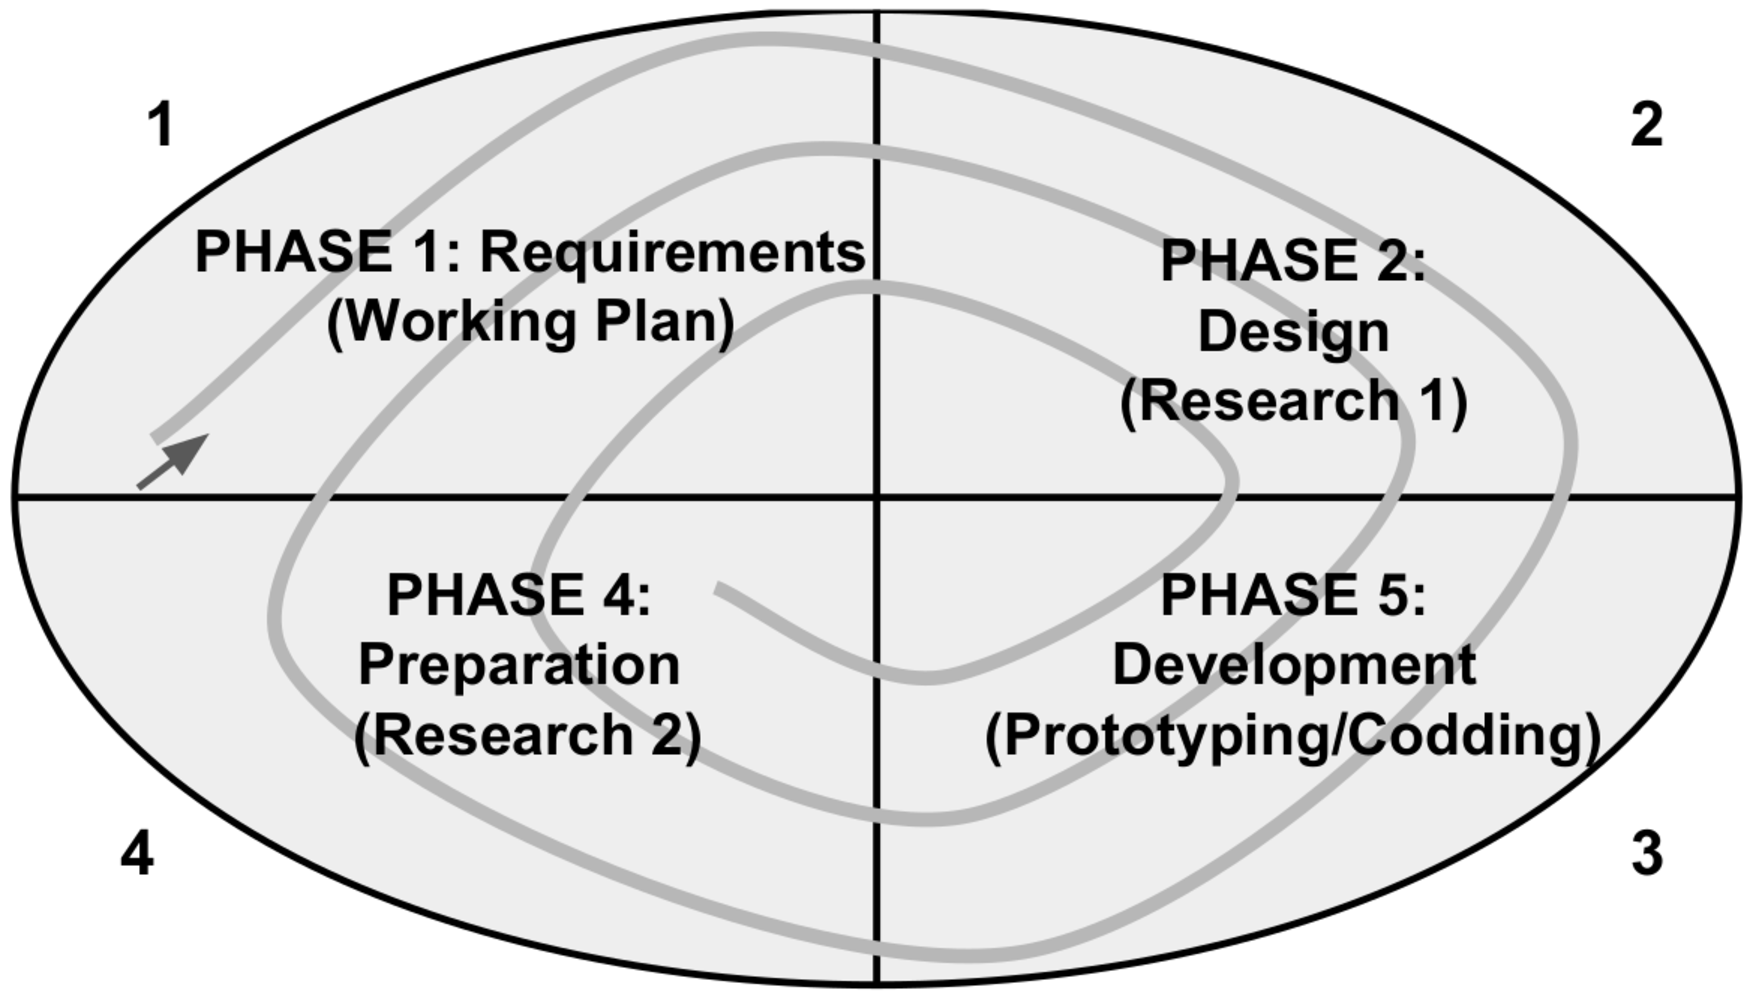
\includegraphics[scale=0.4]{figures/ch1/dev-cicle}
    \caption{Spiral research and development procedure}
    \label{fig:dev-cicle}
\end{figure}

We have adopted a spiral procedure of development, as suggested Sommerville on \textit{Software Engineering}\cite{sommerville}, but adapted to an academic research process. Figure ~\ref{fig:dev-cicle} shows the model of development we had adopted. It had four main phases: 

\begin{enumerate}
    \item \textit{Requirements (Working Plan)};
    \item \textit{Design (research 1)};
    \item \textit{Development (prototyping/codding)};
    \item \textit{Preparation (research 2)}.
\end{enumerate}

On the \textbf{Requirements phase}, we create tasks,  formalized on \textit{Working Plans} documents.  These tasks should cover the whole process. On the \textbf{Design (research 1) phase}, where the focus of the research are related works. We research on literature to learn about topics defined by the task, to help we design our solutions. On this step, during the initial phases of the project,  we also conceived the architecture along with \acrfull{UML} diagrams\footnote{Unified Modeling Language (UML) is a modeling language designed to provide a standardized way of representing and design systems\cite{uml}.}. Some small changes are inevitable, but structural changes turn to be impractical on later phases. The next phase is the \textbf{Development phase}. It is the prototyping and coding phase.  The last is the \textbf{Preparation phase} when we evaluate the results achieved on the Development phase, and we go back to research again,  aiming to prepare the next \textit{Working Plan}.  On this phase, the focus of the research is on points of innovation.


\section{Document Overview}


In this introductory chapter, we had presented an abstract of state of the art, and the main goals of our research. \textit{\textbf{Chapter~\ref{ch:literature-review}}} presents an extensive survey on open-source traffic generator tools, summarizing the benefits, and features supported by each one. The chapter offers a  review of topics on realistic traffic generation and defines important concepts on network traffic modeling; such as self-similarity and heavy-tailed distributions. Also, the chapter presents a survey on techniques for validating traffic generator tools 

\textit{\textbf{Chapter~\ref{ch:architecture}}} presents \textit{SIMITAR} traffic generator. We describe its low-level requirements and define an architecture and their algorithms.  We explain its operation and suggest some use cases. In \textit{\textbf{Chapter~\ref{ch:modeling-evaluation}}} we go deep on the modeling process we had developed for our traffic generator. We validate the effectiveness of Information Criteria \acrfull{AIC} and \acrfull{BIC} as a method selection of stochastic models for  Ethernet traffic.  We also discuss some other algorithms we developed such as \textit{calcOnOff} and the application protocol guesser. In \textit{\textbf{Chapter~\ref{ch:validation}}}, we define a set of metrics based on previous tests on validation of traffic generators found in the literature. Here, we focus on the packet, flow, and scaling metrics. We test our tool in an emulated SDN testbed with Mininet\cite{web-mininet}\footnote{Mininet is a network emulator. It can run a collection of  hosts, switches, routers and links over a single Linux kernel, using lightweight virtualization\cite{web-mininet-repo}.}, using OpenDayLight\cite{web-opendaylight} as a controller. 

\textit{\textbf{Chapter~\ref{ch:future-work}}}  highlights future actions to improve SIMITAR on realism and performance along with other future research avenues, including improving its computational performance, expand it to new APIs of traffic generation and calibration of its constants. Finally, we end the work presentation with a conclusion( \textit{\textbf{chapter~\ref{ch:conclusion}}}).